\documentclass[letterpaper,12pt]{article}
\usepackage{array}
\usepackage{threeparttable}
\usepackage{fancyhdr,lastpage}
\pagestyle{fancy}
\lhead{}
\chead{}
\rhead{}
\lfoot{}
\cfoot{}
\rfoot{\footnotesize\textsl{Page \thepage\ of \pageref{LastPage}}}
\renewcommand\headrulewidth{0pt}
\renewcommand\footrulewidth{0pt}
\usepackage[format=hang,font=normalsize,labelfont=bf]{caption}
\usepackage{listings}
\lstset{frame=single,
  language=Python,
  showstringspaces=false,
  columns=flexible,
  basicstyle={\small\ttfamily},
  numbers=none,
  breaklines=true,
  breakatwhitespace=true
  tabsize=3
}

\usepackage{geometry}
\geometry{letterpaper,tmargin=1in,bmargin=1in,lmargin=1in,rmargin=1in}
%\renewcommand\headrulewidth{2pt}
%\renewcommand\footrulewidth{2pt}
\usepackage{amsmath}
\usepackage{amssymb}
\usepackage{amsthm}
\usepackage{mathtools}
\usepackage{pdflscape}
\usepackage{harvard}
\usepackage{setspace}
\usepackage{float,color}
%\usepackage{enumitem}
\usepackage[pdftex]{graphicx}
\usepackage{hyperref}
\hypersetup{colorlinks,linkcolor=red,urlcolor=blue}
\theoremstyle{definition}
\newtheorem{theorem}{Theorem}
\newtheorem{acknowledgement}[theorem]{Acknowledgement}
\newtheorem{algorithm}[theorem]{Algorithm}
\newtheorem{axiom}[theorem]{Axiom}
\newtheorem{case}[theorem]{Case}
\newtheorem{claim}[theorem]{Claim}
\newtheorem{conclusion}[theorem]{Conclusion}
\newtheorem{condition}[theorem]{Condition}
\newtheorem{conjecture}[theorem]{Conjecture}
\newtheorem{corollary}[theorem]{Corollary}
\newtheorem{criterion}[theorem]{Criterion}
\newtheorem{definition}[theorem]{Definition}
\newtheorem{derivation}{Derivation} % Number derivations on their own
\newtheorem{example}[theorem]{Example}
\newtheorem{exercise}[theorem]{Exercise}
\newtheorem{lemma}[theorem]{Lemma}
\newtheorem{notation}[theorem]{Notation}
\newtheorem{problem}[theorem]{Problem}
\newtheorem{proposition}{Proposition} % Number propositions on their own
\newtheorem{remark}[theorem]{Remark}
\newtheorem{solution}[theorem]{Solution}
\newtheorem{summary}[theorem]{Summary}
\numberwithin{equation}{section}
\bibliographystyle{aer}
\newcommand\ve{\varepsilon}
\newcommand\boldline{\arrayrulewidth{1pt}\hline}
\newcommand{\q}[1]{``#1''}

\def\changemargin#1#2{\list{}{\rightmargin#2\leftmargin#1}\item[]}
\let\endchangemargin=\endlist 

\usepackage{graphicx}
\graphicspath{ {images/} }

\usepackage{enumerate}
%\usepackage[shortlabels]{enumerate}
\setlength{\parindent}{24pt}
%\renewcommand{\baselinestretch}{2.0}
\usepackage{lipsum} % just for the example
\makeatletter
\newcommand{\verbatimfont}[1]{\renewcommand{\verbatim@font}{\ttfamily#1}}
\makeatother
%\usepackage{enumitem}
\usepackage{float}

\verbatimfont{\small}%


\begin{document}

\begin{flushleft}
   \textbf{\Large{Problem Set \#3}} \\
   MACSS 30100 \\
   Luxi Han, 10449918\\
\end{flushleft}

\textbf{[Note]: The \(\mu\) and \(\sigma\) in the legend plotted here is the expectation and standard deviation of the log normal pdf. It is NOT the mean and standard deviation of the income distribution!!}\, \, \\
\, \\

\noindent \textbf{\large Problem 1}\par

\begin{enumerate} [\bfseries (a)]
\item The following graph is the histogram for the income of the MACSS cohort:\\
	\begin{figure}[H]
    		\centering
		\fbox{\resizebox{4.75in}{3in}{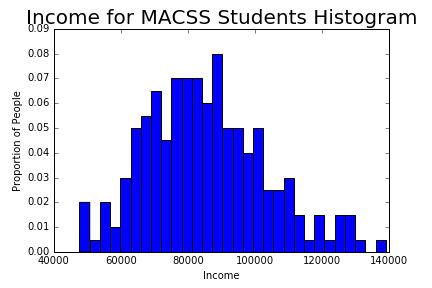
\includegraphics{hist_income}}}\
    		\caption{Histogram of Income of MACSS Students}
	\end{figure}\par
\item \quad
\item The GMM estimator of two moment conditions: the log normal parameters are: \(\mu = 11.331, \, \sigma = 0.209\). \\
	\begin{figure}[H]
    		\centering
		\fbox{\resizebox{5in}{3in}{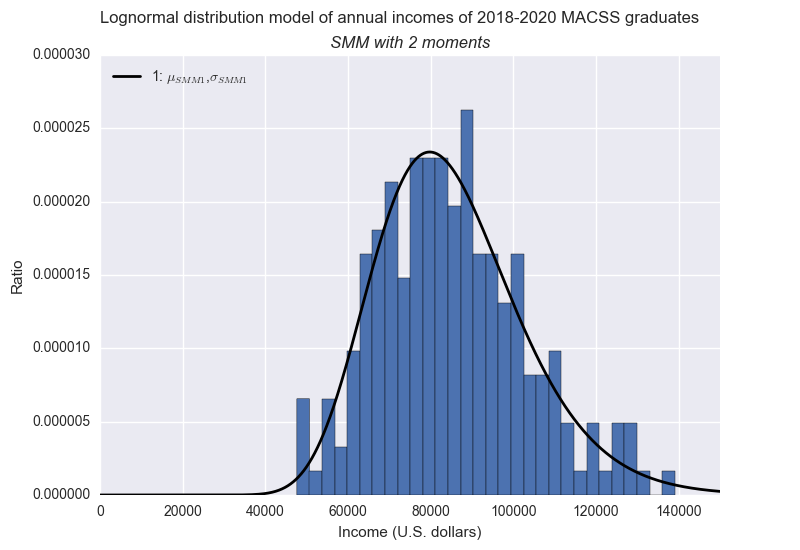
\includegraphics{1c}}}\
    		\caption{Income PDF of SMM(One Step)}
	\end{figure}\par

\item The GMM estimator of two moment conditions using TWO-STEP variance covariance matrix is: the log normal parameters are: \(\mu = 11.330, \, \sigma = 0.209\). \\
The plotted graph is as following:\\
	\begin{figure}[H]
    		\centering
		\fbox{\resizebox{5in}{3in}{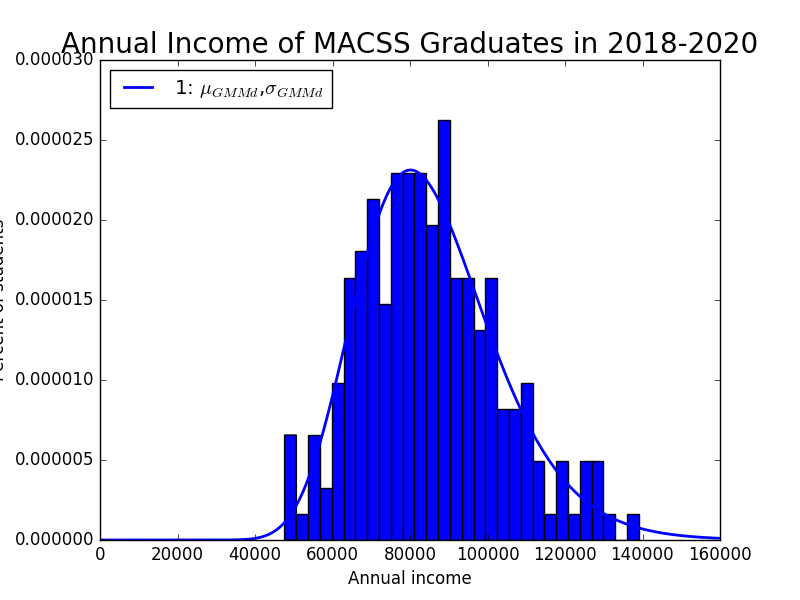
\includegraphics{1d}}}\
    		\caption{Income PDF of SMM(TWO-STEP)}
	\end{figure}\par
We take exponential of the estimated expectation and standard deviation. Then we get:
The data moment is: \(\mu_{data} = 85276.824, \, \sigma_{data} = 17992.542\).\\
\textbf{For ONE Step estimation:}\par
The model moment is \(\mu_{model} = 85134.858, \, \sigma_{model} = 17975.070\)\\
The value of the criterion function is \(8.11793150e-13\)\par
\textbf{For TWO Step estimation:}\par
The model moment is \(\mu_{TWO\_STEP} = 85180.563, \, \sigma_{TWO\_STEP} = 17987.327\)\\
The value of the criterion function is \(-3.39244544e-09\)\par

The two estimations are similar with each other. They are all close to the sample mean of the data. But again, the one step estimator seems to perform slightly better than the one step estimator. 

\end{enumerate}


\end{document}